% Options for packages loaded elsewhere
\PassOptionsToPackage{unicode}{hyperref}
\PassOptionsToPackage{hyphens}{url}
\PassOptionsToPackage{dvipsnames,svgnames,x11names}{xcolor}
%
\documentclass[
  singlecolumn]{report}

\usepackage{amsmath,amssymb}
\usepackage{iftex}
\ifPDFTeX
  \usepackage[T1]{fontenc}
  \usepackage[utf8]{inputenc}
  \usepackage{textcomp} % provide euro and other symbols
\else % if luatex or xetex
  \usepackage{unicode-math}
  \defaultfontfeatures{Scale=MatchLowercase}
  \defaultfontfeatures[\rmfamily]{Ligatures=TeX,Scale=1}
\fi
\usepackage[]{libertinus}
\ifPDFTeX\else  
    % xetex/luatex font selection
\fi
% Use upquote if available, for straight quotes in verbatim environments
\IfFileExists{upquote.sty}{\usepackage{upquote}}{}
\IfFileExists{microtype.sty}{% use microtype if available
  \usepackage[]{microtype}
  \UseMicrotypeSet[protrusion]{basicmath} % disable protrusion for tt fonts
}{}
\makeatletter
\@ifundefined{KOMAClassName}{% if non-KOMA class
  \IfFileExists{parskip.sty}{%
    \usepackage{parskip}
  }{% else
    \setlength{\parindent}{0pt}
    \setlength{\parskip}{6pt plus 2pt minus 1pt}}
}{% if KOMA class
  \KOMAoptions{parskip=half}}
\makeatother
\usepackage{xcolor}
\usepackage[top=30mm,left=20mm,heightrounded]{geometry}
\setlength{\emergencystretch}{3em} % prevent overfull lines
\setcounter{secnumdepth}{-\maxdimen} % remove section numbering
% Make \paragraph and \subparagraph free-standing
\ifx\paragraph\undefined\else
  \let\oldparagraph\paragraph
  \renewcommand{\paragraph}[1]{\oldparagraph{#1}\mbox{}}
\fi
\ifx\subparagraph\undefined\else
  \let\oldsubparagraph\subparagraph
  \renewcommand{\subparagraph}[1]{\oldsubparagraph{#1}\mbox{}}
\fi


\providecommand{\tightlist}{%
  \setlength{\itemsep}{0pt}\setlength{\parskip}{0pt}}\usepackage{longtable,booktabs,array}
\usepackage{calc} % for calculating minipage widths
% Correct order of tables after \paragraph or \subparagraph
\usepackage{etoolbox}
\makeatletter
\patchcmd\longtable{\par}{\if@noskipsec\mbox{}\fi\par}{}{}
\makeatother
% Allow footnotes in longtable head/foot
\IfFileExists{footnotehyper.sty}{\usepackage{footnotehyper}}{\usepackage{footnote}}
\makesavenoteenv{longtable}
\usepackage{graphicx}
\makeatletter
\def\maxwidth{\ifdim\Gin@nat@width>\linewidth\linewidth\else\Gin@nat@width\fi}
\def\maxheight{\ifdim\Gin@nat@height>\textheight\textheight\else\Gin@nat@height\fi}
\makeatother
% Scale images if necessary, so that they will not overflow the page
% margins by default, and it is still possible to overwrite the defaults
% using explicit options in \includegraphics[width, height, ...]{}
\setkeys{Gin}{width=\maxwidth,height=\maxheight,keepaspectratio}
% Set default figure placement to htbp
\makeatletter
\def\fps@figure{htbp}
\makeatother
\newlength{\cslhangindent}
\setlength{\cslhangindent}{1.5em}
\newlength{\csllabelwidth}
\setlength{\csllabelwidth}{3em}
\newlength{\cslentryspacingunit} % times entry-spacing
\setlength{\cslentryspacingunit}{\parskip}
\newenvironment{CSLReferences}[2] % #1 hanging-ident, #2 entry spacing
 {% don't indent paragraphs
  \setlength{\parindent}{0pt}
  % turn on hanging indent if param 1 is 1
  \ifodd #1
  \let\oldpar\par
  \def\par{\hangindent=\cslhangindent\oldpar}
  \fi
  % set entry spacing
  \setlength{\parskip}{#2\cslentryspacingunit}
 }%
 {}
\usepackage{calc}
\newcommand{\CSLBlock}[1]{#1\hfill\break}
\newcommand{\CSLLeftMargin}[1]{\parbox[t]{\csllabelwidth}{#1}}
\newcommand{\CSLRightInline}[1]{\parbox[t]{\linewidth - \csllabelwidth}{#1}\break}
\newcommand{\CSLIndent}[1]{\hspace{\cslhangindent}#1}

\usepackage{booktabs}
\usepackage{longtable}
\usepackage{array}
\usepackage{multirow}
\usepackage{wrapfig}
\usepackage{float}
\usepackage{colortbl}
\usepackage{pdflscape}
\usepackage{tabu}
\usepackage{threeparttable}
\usepackage{threeparttablex}
\usepackage[normalem]{ulem}
\usepackage{makecell}
\usepackage{xcolor}
\makeatletter
\makeatother
\makeatletter
\makeatother
\makeatletter
\@ifpackageloaded{caption}{}{\usepackage{caption}}
\AtBeginDocument{%
\ifdefined\contentsname
  \renewcommand*\contentsname{Table of contents}
\else
  \newcommand\contentsname{Table of contents}
\fi
\ifdefined\listfigurename
  \renewcommand*\listfigurename{List of Figures}
\else
  \newcommand\listfigurename{List of Figures}
\fi
\ifdefined\listtablename
  \renewcommand*\listtablename{List of Tables}
\else
  \newcommand\listtablename{List of Tables}
\fi
\ifdefined\figurename
  \renewcommand*\figurename{Figure}
\else
  \newcommand\figurename{Figure}
\fi
\ifdefined\tablename
  \renewcommand*\tablename{Table}
\else
  \newcommand\tablename{Table}
\fi
}
\@ifpackageloaded{float}{}{\usepackage{float}}
\floatstyle{ruled}
\@ifundefined{c@chapter}{\newfloat{codelisting}{h}{lop}}{\newfloat{codelisting}{h}{lop}[chapter]}
\floatname{codelisting}{Listing}
\newcommand*\listoflistings{\listof{codelisting}{List of Listings}}
\makeatother
\makeatletter
\@ifpackageloaded{caption}{}{\usepackage{caption}}
\@ifpackageloaded{subcaption}{}{\usepackage{subcaption}}
\makeatother
\makeatletter
\@ifpackageloaded{tcolorbox}{}{\usepackage[skins,breakable]{tcolorbox}}
\makeatother
\makeatletter
\@ifundefined{shadecolor}{\definecolor{shadecolor}{rgb}{.97, .97, .97}}
\makeatother
\makeatletter
\makeatother
\makeatletter
\@ifpackageloaded{sidenotes}{}{\usepackage{sidenotes}}
\@ifpackageloaded{marginnote}{}{\usepackage{marginnote}}
\makeatother
\makeatletter
\makeatother
\ifLuaTeX
  \usepackage{selnolig}  % disable illegal ligatures
\fi
\IfFileExists{bookmark.sty}{\usepackage{bookmark}}{\usepackage{hyperref}}
\IfFileExists{xurl.sty}{\usepackage{xurl}}{} % add URL line breaks if available
\urlstyle{same} % disable monospaced font for URLs
\hypersetup{
  pdftitle={Exploring Institutional Trust in New Zealand Pre/Post COVID-19 Pandemic},
  pdfauthor={Authors TBA; Chris G Sibley; Joseph Bulbulia},
  colorlinks=true,
  linkcolor={blue},
  filecolor={Maroon},
  citecolor={Blue},
  urlcolor={Blue},
  pdfcreator={LaTeX via pandoc}}

\title{Exploring Institutional Trust in New Zealand Pre/Post COVID-19
Pandemic}
\usepackage{etoolbox}
\makeatletter
\providecommand{\subtitle}[1]{% add subtitle to \maketitle
  \apptocmd{\@title}{\par {\large #1 \par}}{}{}
}
\makeatother
\subtitle{New Zealand Attitudes and Values Study: Years 2019-2022 N =
42,681}
\author{Authors TBA \and Chris G Sibley \and Joseph Bulbulia}
\date{2023-03-23}

\begin{document}
\maketitle
\ifdefined\Shaded\renewenvironment{Shaded}{\begin{tcolorbox}[boxrule=0pt, borderline west={3pt}{0pt}{shadecolor}, breakable, enhanced, sharp corners, interior hidden, frame hidden]}{\end{tcolorbox}}\fi

\listoffigures
\listoftables
\hypertarget{nzavs-report-on-institutional-trust-prepost-covid}{%
\section{NZAVS Report on Institutional Trust Pre/Post
COVID}\label{nzavs-report-on-institutional-trust-prepost-covid}}

This report delves into the changes in institutional trust among New
Zealanders from the pre-pandemic period in 2019 to 2022.

The New Zealand Attitudes and Values Study uses a two-item scale to
measure \textbf{Trust in Science}

\begin{itemize}
\item
  ``I have a high degree of confidence in the scientific
  community.''(\protect\hyperlink{ref-nisbet2015}{Nisbet, Cooper, and
  Garrett 2015})
\item
  ``Our society places too much emphasis on science.''(reverse coded)
\end{itemize}

We average these scores to form a single score
(\protect\hyperlink{ref-hartman2017}{Hartman et al. 2017}). \footnote{We
  do not blindly adhere to the standard measurement approaches in
  psychometrics. It might be preferable to work with single items
  instead of the averaged score. See
  (\protect\hyperlink{ref-vanderweele2022}{VanderWeele 2022}) for more
  information on this point.} These items were introduced in NZAVS Wave
11 (2019 - 2020) \footnote{We must be cautious: causal identification
  requires contrasting outcomes under different exposures. Because all
  were exposed to the COVID-19 pandemic, these contrasts are not
  identified without the strong assumption that there were no
  pre-existing trends in the acceptance of science before the COVID-19
  pandemic struck.}

Previous research using a propensity score design reported on changes in
Trust in Science during the first three weeks of New Zealand's COVID
lockdown in March and April 2020
(\protect\hyperlink{ref-sibley2020}{Sibley et al. 2020}).

\textbf{COVID-19 Government response}
(\protect\hyperlink{ref-marques2022}{Marques et al. 2022})

\begin{itemize}
\tightlist
\item
  ``I trust the Government to make sensible decisions about how to best
  manage COVID-19 in New Zealand.''
\item
  ``The New Zealand government response to COVID-19.''
\end{itemize}

\textbf{Trust in politicians} (\protect\hyperlink{ref-sibley2020}{Sibley
et al. 2020})

\begin{itemize}
\tightlist
\item
  ``Politicians in New Zealand can generally be trusted.''
\end{itemize}

\textbf{Institutional trust in police}
(\protect\hyperlink{ref-tyler2005}{Tyler 2005})

\begin{itemize}
\tightlist
\item
  ``People's basic rights are well protected by the New Zealand
  Police.''
\item
  ``There are many things about the New Zealand Police and its policies
  that need to be changed.''
\item
  ``The New Zealand Police care about the well-being of everyone they
  deal with.''
\end{itemize}

\textbf{General tendency to believe in
conspiracies}(\protect\hyperlink{ref-lantian2016}{Lantian et al. 2016})

\begin{itemize}
\tightlist
\item
  ``I think that the official version of major world events given by
  authorities often hides the truth.''
\end{itemize}

\hypertarget{sample-responses-years-2019-2020-pre-covid-lockdown-post-lockdown}{%
\subsection{Sample responses: years 2019-2020: Pre-Covid, Lockdown,
Post-Lockdown}\label{sample-responses-years-2019-2020-pre-covid-lockdown-post-lockdown}}

\begin{longtable}[]{@{}
  >{\raggedright\arraybackslash}p{(\columnwidth - 6\tabcolsep) * \real{0.3152}}
  >{\raggedright\arraybackslash}p{(\columnwidth - 6\tabcolsep) * \real{0.2283}}
  >{\raggedright\arraybackslash}p{(\columnwidth - 6\tabcolsep) * \real{0.2283}}
  >{\raggedright\arraybackslash}p{(\columnwidth - 6\tabcolsep) * \real{0.2283}}@{}}
\toprule\noalign{}
\begin{minipage}[b]{\linewidth}\raggedright
Forms of Institutional Trust
\end{minipage} & \begin{minipage}[b]{\linewidth}\raggedright
pre\_covid
\end{minipage} & \begin{minipage}[b]{\linewidth}\raggedright
lockdown
\end{minipage} & \begin{minipage}[b]{\linewidth}\raggedright
post\_lockdown
\end{minipage} \\
\midrule\noalign{}
\endhead
\bottomrule\noalign{}
\endlastfoot
& (N=29812) & (N=3511) & (N=9358) \\
Trust\_in\_Science & & & \\
Mean (SD) & 5.36 (± 1.28) & 5.66 (± 1.23) & 5.55 (± 1.27) \\
Missing & 289 (1.0\%) & 16 (0.5\%) & 70 (0.7\%) \\
Trust\_in\_Politicians & & & \\
Mean (SD) & 3.72 (± 1.44) & 4.00 (± 1.48) & 3.78 (± 1.48) \\
Missing & 685 (2.3\%) & 25 (0.7\%) & 143 (1.5\%) \\
Trust\_in\_Police & & & \\
Mean (SD) & 4.61 (± 1.23) & 4.60 (± 1.34) & 4.50 (± 1.33) \\
Missing & 12 (0.0\%) & 0 (0\%) & 3 (0.0\%) \\
Conspiracy\_Beliefs & & & \\
Mean (SD) & 4.38 (± 1.60) & 4.29 (± 1.68) & 4.31 (± 1.69) \\
Missing & 940 (3.2\%) & 43 (1.2\%) & 214 (2.3\%) \\
\end{longtable}

Here is a graph of the same.

\begin{figure}

{\centering 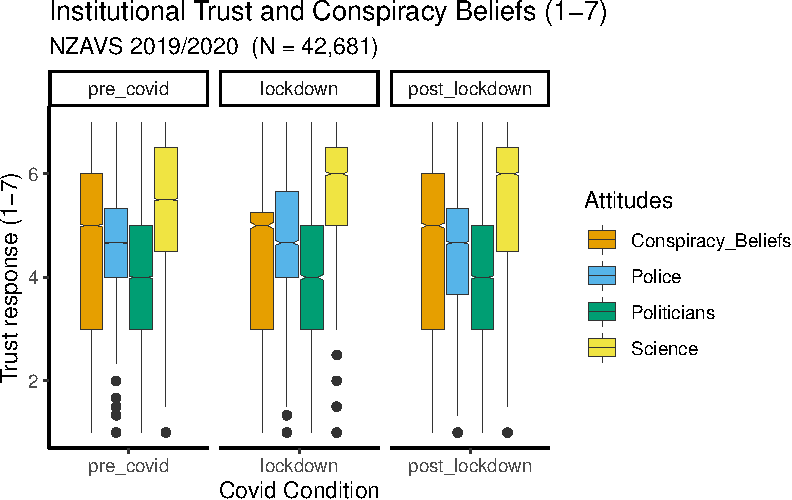
\includegraphics{trust-science_files/figure-pdf/fig-trust-wave-11-1.pdf}

}

\caption{\label{fig-trust-wave-11}Boxplot for Institutional Trust: NZAVS
Waves During Covid: Years 2020}

\end{figure}

This table and graph compare the trust in science, police, and
politicians across three different periods: pre-Covid, lockdown, and
post-lockdown.

We observe:

\begin{enumerate}
\def\labelenumi{\arabic{enumi}.}
\tightlist
\item
  Trust in science increased during the lockdown period and remained
  higher in the post-lockdown period compared to the pre-Covid period.
\item
  Trust in police remained relatively stable across all three periods,
  although the trend tracked downward after lockdown.
\item
  Trust in politicians increased during the lockdown period. It
  decreased slightly in the post-lockdown period but remained higher
  than in the pre-Covid period.
\item
  Conspiracy Beliefs: the average mistrust of official versions of major
  world events given by authorities appear to decrease during lockdown
  but subsequently decrease.
\end{enumerate}

Notably, the central tendency may not always be the interesting
statistic for understanding social change. There may be greater
galvanisation in response that is masked by overall average response. In
future work, we will examine this point. For now, the trends suggest
overall stability during 2019-2020, with increasing confidence in
science.

\hypertarget{nzavs-sample-responses-years-2019-2022}{%
\subsection{NZAVS sample responses: years
2019-2022}\label{nzavs-sample-responses-years-2019-2022}}

Next, we examine changes in institutional trust across two waves
following the 2019/2020 NZAVS wave.

Table:

\begin{longtable}[]{@{}
  >{\raggedright\arraybackslash}p{(\columnwidth - 6\tabcolsep) * \real{0.3152}}
  >{\raggedright\arraybackslash}p{(\columnwidth - 6\tabcolsep) * \real{0.2283}}
  >{\raggedright\arraybackslash}p{(\columnwidth - 6\tabcolsep) * \real{0.2283}}
  >{\raggedright\arraybackslash}p{(\columnwidth - 6\tabcolsep) * \real{0.2283}}@{}}
\toprule\noalign{}
\begin{minipage}[b]{\linewidth}\raggedright
Forms of Institutional Trust
\end{minipage} & \begin{minipage}[b]{\linewidth}\raggedright
X2019
\end{minipage} & \begin{minipage}[b]{\linewidth}\raggedright
X2020
\end{minipage} & \begin{minipage}[b]{\linewidth}\raggedright
X2021
\end{minipage} \\
\midrule\noalign{}
\endhead
\bottomrule\noalign{}
\endlastfoot
& (N=42681) & (N=42681) & (N=42681) \\
Trust\_in\_Science & & & \\
Mean (SD) & 5.43 (± 1.28) & 5.67 (± 1.24) & 5.70 (± 1.26) \\
Missing & 375 (0.9\%) & 9475 (22.2\%) & 14231 (33.3\%) \\
Trust\_in\_Politicians & & & \\
Mean (SD) & 3.76 (± 1.45) & 4.05 (± 1.49) & 3.92 (± 1.56) \\
Missing & 853 (2.0\%) & 10078 (23.6\%) & 15406 (36.1\%) \\
Trust\_in\_Police & & & \\
Mean (SD) & 4.58 (± 1.26) & 4.53 (± 1.26) & 4.43 (± 1.30) \\
Missing & 15 (0.0\%) & 9378 (22.0\%) & 13770 (32.3\%) \\
Trust\_in\_Govt\_Covid\_Response & & & \\
Mean (SD) & NA (± NA) & 5.66 (± 1.55) & 4.79 (± 1.94) \\
Missing & 42681 (100\%) & 9620 (22.5\%) & 15123 (35.4\%) \\
Conspiracy\_Beliefs & & & \\
Mean (SD) & 4.36 (± 1.63) & 4.10 (± 1.68) & 4.02 (± 1.74) \\
Missing & 1197 (2.8\%) & 9676 (22.7\%) & 15110 (35.4\%) \\
\end{longtable}

Here is a graph of the same.

\begin{figure}

{\centering 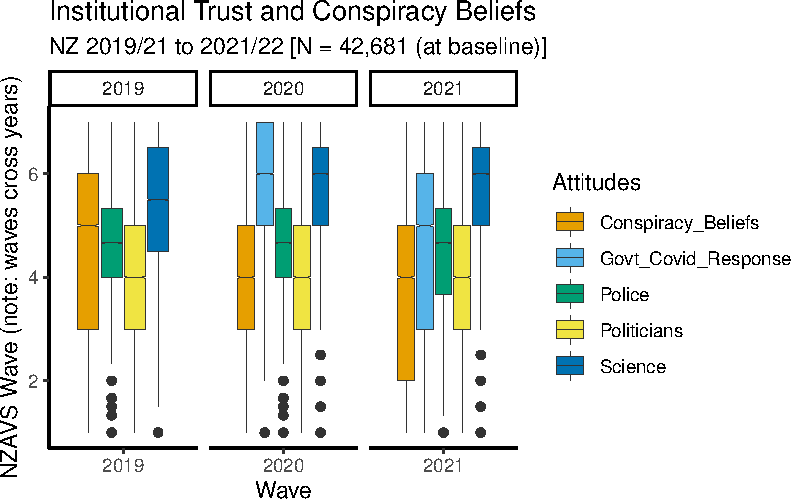
\includegraphics{trust-science_files/figure-pdf/fig-trust-1.pdf}

}

\caption{\label{fig-trust}Boxplot for Institutional Trust: NZAVS Waves
11-13 (years 2019-2022)}

\end{figure}

Descriptive fndings.

Trust in Science: The average trust score increased from 5.43 (±1.28) in
2019 to 5.67 (±1.24) in 2020 and to 5.70 (±1.26) in 2021. The number of
missing values increased from 375 (0.9\%) in 2019 to 9,475 (22.2\%) in
2020 and further to 14,231 (33.3\%) in 2021.

Trust in Politicians: The average trust score increased from 3.76
(±1.45) in 2019 to 4.05 (±1.49) in 2020, then slightly decreased to 3.92
(±1.56) in 2021. The number of missing values increased from 853 (2.0\%)
in 2019 to 10,078 (23.6\%) in 2020 and further to 15,406 (36.1\%) in
2021.

Trust in Police: The average trust score decreased from 4.58 (±1.26) in
2019 to 4.53 (±1.26) in 2020 and further to 4.43 (±1.30) in 2021. The
number of missing values increased from 15 (0.0\%) in 2019 to 9,378
(22.0\%) in 2020 and further to 13,770 (32.3\%) in 2021.

Trust in Government's COVID Response: This metric was not applicable in
2019. The average trust score was 5.66 (±1.55) in 2020 and decreased to
4.79 (±1.94) in 2021. The number of missing values was 42,681 (100\%) in
2019, 9,620 (22.5\%) in 2020, and 15,123 (35.4\%) in 2021.

Conspiracy Beliefs: The average score decreased from 4.36 (±1.63) in
2019 to 4.10 (±1.68) in 2020 and further to 4.02 (±1.74) in 2021. The
number of missing values increased from 1,197 (2.8\%) in 2019 to 9,676
(22.7\%) in 2020 and further to 15,110 (35.4\%) in 2021.

How should we in interpret these findings? Missing data from
non-response and panel attrition may bias estimates for the population.
We must address bias from missing responses. We address this bias
through multiple imputation.

\hypertarget{handling-missingness}{%
\section{Handling missingness}\label{handling-missingness}}

To handle missing data, we must model and predict missing responses. We
attempt two types of missing data imputation. Both use machine learning.
The first is the \texttt{mlim} package in R, which uses model tuning to
optimise the prediction of missing values. The second is the
\texttt{mice} package in R. It uses predictive mean matching (ppm)
optimse the prediction of missing values. We find that the mice
package/ppm performs better, and present the\texttt{ppm} results here.
We present the code for both approaches below.

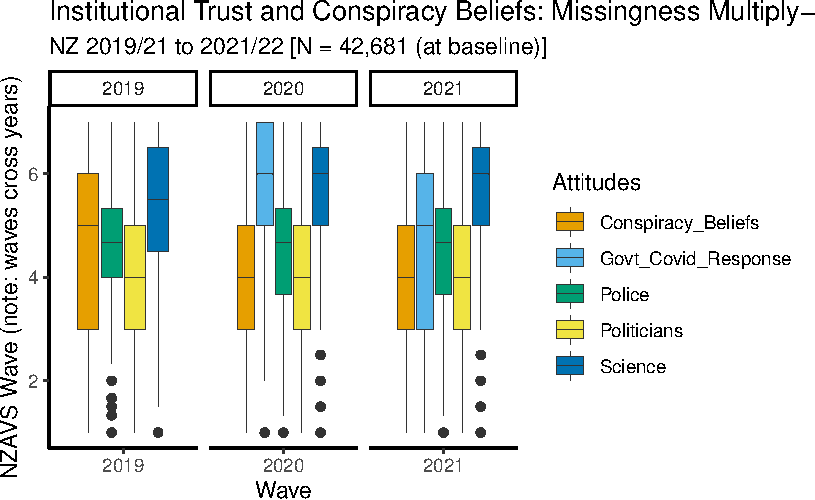
\includegraphics{trust-science_files/figure-pdf/ppm-graph-1.pdf}

\begin{longtable}[]{@{}
  >{\raggedright\arraybackslash}p{(\columnwidth - 6\tabcolsep) * \real{0.3152}}
  >{\raggedright\arraybackslash}p{(\columnwidth - 6\tabcolsep) * \real{0.2283}}
  >{\raggedright\arraybackslash}p{(\columnwidth - 6\tabcolsep) * \real{0.2283}}
  >{\raggedright\arraybackslash}p{(\columnwidth - 6\tabcolsep) * \real{0.2283}}@{}}
\toprule\noalign{}
\begin{minipage}[b]{\linewidth}\raggedright
Forms of Institutional Trust
\end{minipage} & \begin{minipage}[b]{\linewidth}\raggedright
X2019
\end{minipage} & \begin{minipage}[b]{\linewidth}\raggedright
X2020
\end{minipage} & \begin{minipage}[b]{\linewidth}\raggedright
X2021
\end{minipage} \\
\midrule\noalign{}
\endhead
\bottomrule\noalign{}
\endlastfoot
& (N=469491) & (N=469491) & (N=469491) \\
Trust\_in\_Science & & & \\
Mean (SD) & 5.43 (± 1.28) & 5.64 (± 1.25) & 5.65 (± 1.28) \\
Missing & 375 (0.1\%) & 9475 (2.0\%) & 14231 (3.0\%) \\
Trust\_in\_Politicians & & & \\
Mean (SD) & 3.76 (± 1.45) & 4.02 (± 1.50) & 3.85 (± 1.57) \\
Missing & 853 (0.2\%) & 10078 (2.1\%) & 15406 (3.3\%) \\
Trust\_in\_Police & & & \\
Mean (SD) & 4.58 (± 1.26) & 4.50 (± 1.27) & 4.37 (± 1.32) \\
Missing & 15 (0.0\%) & 9378 (2.0\%) & 13770 (2.9\%) \\
Trust\_in\_Govt\_Covid\_Response & & & \\
Mean (SD) & NA (± NA) & 5.64 (± 1.56) & 4.74 (± 1.96) \\
Missing & 469491 (100\%) & 9620 (2.0\%) & 15123 (3.2\%) \\
Conspiracy\_Beliefs & & & \\
Mean (SD) & 4.36 (± 1.63) & 4.13 (± 1.68) & 4.06 (± 1.75) \\
Missing & 1197 (0.3\%) & 9676 (2.1\%) & 15110 (3.2\%) \\
\end{longtable}

The imputed data contain ten imputed datasets plus the original data
with missing values. We will need to adjust for the uncertainities of
multiple imputation using Rubin's rule.

Additionally, we are now grouping pre and post responses together in the
2019 wave. So we are no longer identifying specific responses of to the
COVID pandemic and response. To identify the specific effects of the
COVID pandemic and response requires care. There are no contrasts from
which to derive comparisons. That is, because all in the population were
subject to the exposure, we cannot straightforwardly infer how people
would have responded were they not exposed. We will return to this issue
in future work.

These provisos aside, we find evidence for continued average confidence
in science, with some evidence for a continued downward shift in trust
for the NZ police.

Next, we formally model change over time using generalised estimating
equations (GEE). They models take into account uncertainties from
multiple imputation. We employ survey weights to recover population
estimates.

\hypertarget{results-for-average-responses.}{%
\subsection{Results for average
responses.}\label{results-for-average-responses.}}

\hypertarget{trust-in-science}{%
\subsection{Trust in science}\label{trust-in-science}}

\begin{longtable}[]{@{}lrrrrr@{}}
\caption{Trust in Science by NZAVS Wave }\tabularnewline
\toprule\noalign{}
term & estimate & std.error & statistic & df & p.value \\
\midrule\noalign{}
\endfirsthead
\toprule\noalign{}
term & estimate & std.error & statistic & df & p.value \\
\midrule\noalign{}
\endhead
\bottomrule\noalign{}
\endlastfoot
(Intercept) & 5.451 & 0.007 & 756.404 & 62762.541 & 0 \\
Wave2020 & 0.192 & 0.006 & 29.781 & 176.552 & 0 \\
Wave2021 & 0.215 & 0.007 & 29.572 & 146.591 & 0 \\
\end{longtable}

\begin{longtable}[]{@{}lrrrrr@{}}
\caption{Trust in Politicians by NZAVS Wave }\tabularnewline
\toprule\noalign{}
term & estimate & std.error & statistic & df & p.value \\
\midrule\noalign{}
\endfirsthead
\toprule\noalign{}
term & estimate & std.error & statistic & df & p.value \\
\midrule\noalign{}
\endhead
\bottomrule\noalign{}
\endlastfoot
(Intercept) & 3.736 & 0.008 & 441.327 & 14871.025 & 0 \\
Wave2020 & 0.251 & 0.009 & 28.251 & 93.102 & 0 \\
Wave2021 & 0.080 & 0.009 & 8.803 & 259.975 & 0 \\
\end{longtable}

\begin{longtable}[]{@{}lrrrrr@{}}
\caption{Trust in Police by NZAVS Wave }\tabularnewline
\toprule\noalign{}
term & estimate & std.error & statistic & df & p.value \\
\midrule\noalign{}
\endfirsthead
\toprule\noalign{}
term & estimate & std.error & statistic & df & p.value \\
\midrule\noalign{}
\endhead
\bottomrule\noalign{}
\endlastfoot
(Intercept) & 4.539 & 0.008 & 574.900 & 103491.441 & 0 \\
Wave2020 & -0.110 & 0.007 & -16.752 & 111.240 & 0 \\
Wave2021 & -0.247 & 0.008 & -31.849 & 133.079 & 0 \\
\end{longtable}

\begin{longtable}[]{@{}lrrrrr@{}}
\caption{Trust in Science by NZAVS Wave }\tabularnewline
\toprule\noalign{}
term & estimate & std.error & statistic & df & p.value \\
\midrule\noalign{}
\endfirsthead
\toprule\noalign{}
term & estimate & std.error & statistic & df & p.value \\
\midrule\noalign{}
\endhead
\bottomrule\noalign{}
\endlastfoot
(Intercept) & 5.614 & 0.011 & 523.237 & 103.496 & 0 \\
Wave2021 & -0.903 & 0.011 & -81.429 & 67.518 & 0 \\
\end{longtable}

\begin{longtable}[]{@{}lrrrrr@{}}
\caption{Conspiracy Beliefs by NZAVS Wave }\tabularnewline
\toprule\noalign{}
term & estimate & std.error & statistic & df & p.value \\
\midrule\noalign{}
\endfirsthead
\toprule\noalign{}
term & estimate & std.error & statistic & df & p.value \\
\midrule\noalign{}
\endhead
\bottomrule\noalign{}
\endlastfoot
(Intercept) & 4.362 & 0.009 & 464.975 & 4101.840 & 0 \\
Wave2020 & -0.251 & 0.012 & -20.768 & 49.163 & 0 \\
Wave2021 & -0.308 & 0.013 & -23.368 & 48.228 & 0 \\
\end{longtable}

The results reflect findings in the descriptiove tables.

\hypertarget{trust-in-science-by-nzavs-wave}{%
\subsubsection{Trust in Science by NZAVS
Wave:}\label{trust-in-science-by-nzavs-wave}}

\begin{itemize}
\tightlist
\item
  From 2019 to 2020, trust in science reliably increased (estimate =
  0.192, p \textless{} 0.001).
\item
  From 2019 to 2021, trust in science also reliably increased (estimate
  = 0.215, p \textless{} 0.001).
\end{itemize}

There is no downward trend in average Trust in Science.

\hypertarget{trust-in-politicians-by-nzavs-wave}{%
\subsubsection{Trust in Politicians by NZAVS
Wave:}\label{trust-in-politicians-by-nzavs-wave}}

\begin{itemize}
\tightlist
\item
  From 2019 to 2020, the increase in trust in politicians was reliable
  (estimate = 0.251, p \textless{} 0.001).
\item
  From 2019 to 2021, the increase in trust in politicians was also
  reliable (estimate = 0.080, p \textless{} 0.001).
\end{itemize}

Comparisons here are with the baseline wave, comparing 2019 and 2021 we
find evidence for regression to the baseline wave. Whereas trust in
politicians increased during the initial COVID-19 attack and response,
gains to average trust appear to have been dropping.

\hypertarget{trust-in-police-by-nzavs-wave}{%
\subsubsection{Trust in Police by NZAVS
Wave:}\label{trust-in-police-by-nzavs-wave}}

\begin{itemize}
\tightlist
\item
  From 2019 to 2020, the decrease in trust in police was reliable
  (estimate = -0.110, p \textless{} 0.001).
\item
  From 2019 to 2021, the decrease in trust in police was also reliable
  (estimate = -0.247, p \textless{} 0.001).
\end{itemize}

Here we find evidence for declining Trust in the NZ police. Notably,
however, overall levels of Trust in the NZ police remain high.

\hypertarget{trust-in-government-covid-response-by-nzavs-wave-only-two-waves}{%
\subsubsection{Trust in Government COVID Response by NZAVS Wave (only
two
waves):}\label{trust-in-government-covid-response-by-nzavs-wave-only-two-waves}}

\begin{itemize}
\tightlist
\item
  From 2019 to 2021, the decrease in trust in the NZ government's COVID
  response was reliable (estimate = -0.903, p \textless{} 0.001). This
  represents a major drop in confidence. Notably, this drop in
  confidence for the NZ government's COVID response has not considerably
  affected attitudes to science.
\end{itemize}

\hypertarget{conspiracy-beliefs}{%
\subsubsection{Conspiracy Beliefs:}\label{conspiracy-beliefs}}

\begin{itemize}
\tightlist
\item
  From 2019 to 2020, the decrease in conspiracy beliefs was reliable
  (estimate = -0.251, p \textless{} 0.001).
\item
  From 2019 to 2021, the decrease in conspiracy beliefs was also
  reliable (estimate = -0.308, p \textless{} 0.001).
\end{itemize}

On average, we find that conspiracy beliefs are falling. However, this
evidence is based on the assumptions that the model we have used impute
missing conspiracy beliefs is adequate. It is possible that real change
in conspiracy beliefs, and indeed for all imputed variables differs from
what we have recovered in the imputation model.

\hypertarget{summary}{%
\subsection{Summary}\label{summary}}

The results indicate a reliable increase in trust in science from 2019
to 2020, and that this shift has remained constant. In contrast, changes
in trust in politicians, trust in police, trust in the government's
COVID response, across the waves were generally unreliable. Evidence
suggests that average conspiracy beliefs may have declined.

The preliminary findings merit further research.

Firstly, multiple imputation models rely on assumptions. These
assumptions must be tested.

Secondly, when a population becomes more polarized, the average response
may be misleading, potentially indicating no change. We must investigate
change at the margins of reponse, not merely at the average response.

Thirdly, we need not assume that the items model a univariate latent
construct. We might instead model items from the scales individually, as
suggested by VanderWeele
(\protect\hyperlink{ref-vanderweele2022}{2022}).

In the near future, that address these challenges. Stay tuned!

\hypertarget{information-about-the-new-zealand-attitudes-and-values-study.}{%
\subsection{Information about the New Zealand Attitudes and Values
Study.}\label{information-about-the-new-zealand-attitudes-and-values-study.}}

For more information about the NZAVS see:
\href{https://www.psych.auckland.ac.nz/en/about/new-zealand-attitudes-and-values-study.html}{here}
and \href{https://go-bayes.github.io/reports/posts/nzavs/}{here}

\hypertarget{refs}{}
\begin{CSLReferences}{1}{0}
\leavevmode\vadjust pre{\hypertarget{ref-hartman2017}{}}%
Hartman, Robert O., Nathan F. Dieckmann, Amber M. Sprenger, Bradley J.
Stastny, and Kenneth G. DeMarree. 2017. {``Modeling Attitudes Toward
Science: Development and Validation of the Credibility of Science
Scale.''} \emph{Basic and Applied Social Psychology} 39: 358--71.
\url{https://doi.org/10.1080/01973533.2017.1372284}.

\leavevmode\vadjust pre{\hypertarget{ref-lantian2016}{}}%
Lantian, Anthony, Dominique Muller, Cécile Nurra, and Karen M Douglas.
2016. {``Measuring Belief in Conspiracy Theories: Validation of a French
and English Single-Item Scale.''} \emph{International Review of Social
Psychology} 29 (1): 114.

\leavevmode\vadjust pre{\hypertarget{ref-marques2022}{}}%
Marques, Mathew D, Chris G Sibley, Marc Wilson, Joseph A Bulbulia, Danny
Osborne, Kumar Yogeeswaran, Carol Lee, Isabelle M Duck, Karen Douglas,
and Aleksandra Cichocka. 2022. {``Psychological Predictors of COVID-19
Vaccination in New Zealand.''}

\leavevmode\vadjust pre{\hypertarget{ref-nisbet2015}{}}%
Nisbet, Erik C., Kathryn E. Cooper, and R. Kelly Garrett. 2015. {``The
Partisan Brain: How Dissonant Science Messages Lead Conservatives and
Liberals to (Dis)trust Science.''} \emph{The ANNALS of the American
Academy of Political and Social Science} 658 (1): 36--66.
\url{https://doi.org/10.1177/0002716214555474}.

\leavevmode\vadjust pre{\hypertarget{ref-sibley2020}{}}%
Sibley, Chris G, Lara Greaves, Nicole Satherley, Petar Milojev, Joseph
Bulbulia, Fiona Barlow, Danny Osborne, et al. 2020. {``What Happened to
People in New Zealand During Covid-19 Home Lockdown? Institutional
Trust, Attitudes to Government, Mental Health and Subjective
Wellbeing.''} \href{https://osf.io/e765a}{osf.io/e765a}.

\leavevmode\vadjust pre{\hypertarget{ref-tyler2005}{}}%
Tyler, Tom R. 2005. {``Policing in Black and White: Ethnic Group
Differences in Trust and Confidence in the Police.''} \emph{Police
Quarterly} 8 (3): 322342.

\leavevmode\vadjust pre{\hypertarget{ref-vanderweele2022}{}}%
VanderWeele, Tyler J. 2022. {``Constructed Measures and Causal
Inference: Towards a New Model of Measurement for Psychosocial
Constructs.''} \emph{Epidemiology} 33 (1): 141.
\url{https://doi.org/10.1097/EDE.0000000000001434}.

\end{CSLReferences}



\end{document}
